\section{Image Features and Segmentation}

\subsection{Image Feature Morphology}

Upon feature extraction, feature vectors are a product. The differing morphologies of feature extractor, output a varying numbers of features. \\

\noindent If we were to analyse an image as one, for an output of one featurevector. We would describe this as a \textbf{Global Feature}.

\subsubsection{Grid or Block-based Features}
The image is passed to a feature extractor, the image is split by a $NxN$ grid, and \textbf{one} feature is extracted from \textbf{each block}. 

\subsubsection{Region-based Features}
The image is split into a number of regions, and a feature is extracted for each region. \textbf{One} feature is extracted \textbf{per region}.

\subsubsection{Local Features}
The image is analysed by the feature extractor, points of interest are detected, and as a result a feature is extracted from the surrounding pixels. \textbf{One} feature \textbf{local interest point}.

\subsection{Global Features}
This section details methods and concepts of finding global features within an image.
\subsubsection{Histograms}
\textbf{Image Histograms} A common approach to computing a global image description, is to compute a histogram of the pixel values. \\

\textbf{Joint-colour Histograms} measures the frequency of occurency of each colour in the image. We compute a separate histogram for each channel. The colourspace is quantised into bins, and we accumulate the number pixels in each bin.

\subsection{Segmentation}
Segmentation can be defined as:

\begin{quote}
    The process of partitioning the image into sets of pixels, often called segments. Pixels within a segment often share visual characteristics
\end{quote}

\subsubsection{Global Binary Thresholding}
Thresholding is the simplest form of segmentation.
\begin{itemize}
    \itemsep0em
    \item Turns grey level images into binary images, by assigning pixels with a value less than a threshold to one segment, and other pixels to another.
    \item This method is very fast
    \item Requires a manually set threshold. This is not robust to lighting changes. But works well with constraints.
\end{itemize}

\subsubsection{Otsu's Thresholding Method}
Similar conceptually to global binary thresholding however provides a way to automatically find the threshold.

\begin{itemize}
    \itemsep0em
    \item Assume there are two classes, foreground and background.
    \item Therefore, the histogram must have two peaks.
    \item Exhaustively search the histogram that maximises the interclass value.
\end{itemize}

This is visualised in figure \ref{fig:otsu}

\begin{figure}{!h}
    \centering
    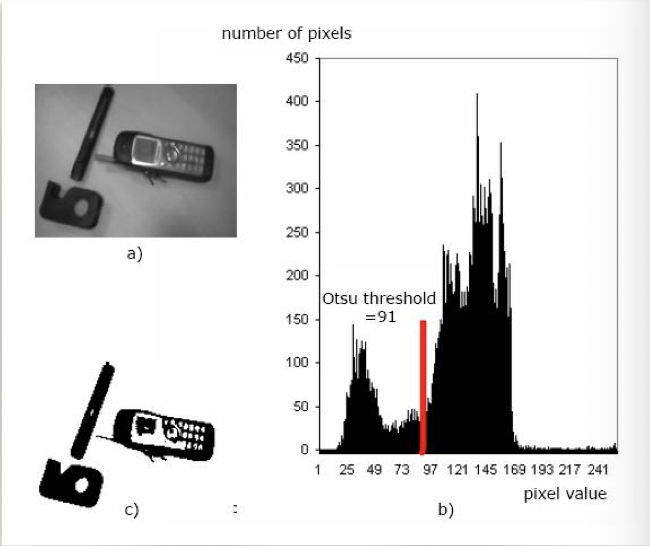
\includegraphics[scale=0.4]{Images/Otsu.png}
    \caption{Otsu Thresholding}
    \label{fig:otsu}
\end{figure}

We can see in the example, that a threshold is found at a pixel value of 91.


\subsection{Local Features}

Local or adaptive thresholding operators compute a different threshold value for every pixel in an image, based on the surrounding pixels. We use a rectangular window around a pixel to define the neighbours.

\subsubsection{Mean Adaptive Thresholding}
The MAT local feature method works as follows:
\begin{itemize}
    \itemsep0em 
    \item [\textbf{Statement}] Set the current pixel to zero if
    \item [\textbf{Condition}] The value is less than the $mean+constant$ of the neighbours in a given window 
    \item [\textbf{Otherwise}] set to one
\end{itemize}

\noindent We can evaluate the pros and cons

\begin{itemize}
    \itemsep0em
    \item [\textbf{Pros}] Good invariance to uneven lighting
    \item Good invariance to a variety of contrasts
    \item [\textbf{Cons}] Computationally expensive as its pixel by pixel
    \item Can be difficult to choose the window size
    \item If the object being imaged can appear at different distances to the camera, then it could break.
\end{itemize}

\subsubsection{Segmentation with K-Means Clustering}
K-Means clustering provides a simple method for performing segmentation.
\\
\noindent We start by clustering the colour vectors of all the pixels, then assign each pixel to a segment based on the closest cluster centroid.

\\

\noindent The Naive approach to segmentation using K-Means doesnt attempt to preserve continuity of segments. This means you end up with pixels assigned to a segment, that are far away from other pixels in that segment.

\\
\noindent Normalise x and y by the width and height of the image to take away the effect of image size.

\subsection{Pixel Connectivity}

A pixel is said to be connected with another if they are spatially adjacent to each other. We can define this by \textit{4-connectivity} and \textit{8-connectivity}.


\begin{figure}{!h}
    \centering
    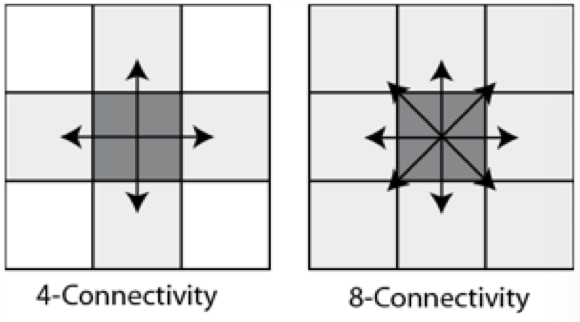
\includegraphics[scale=0.4]{Images/pixcon.png}
    \caption{Pixel Connectivity}
    \label{fig:con}
\end{figure}

A connected component is a set of pixels where every pixel is connected directly or through any connected path from the set.

\subsubsection{Connected Component Labelling}
The process of finding all the connected components within a binary (segmented) image. Where each connected segment is identified as a connected component.
\\

\noindent The two pass algorithm is described below.

\begin{itemize}
    \itemsep0em
    \item [\textbf{1}] On the first pass, iterate through each element of the data by column, then by row:
    \setlength{\itemindent}{.15in}
    \item If the element is not in the background
    \item Get the neighbouring elements of the current element.
    \item If there are no neighbours, uniquely label the current element and continue.
    \item Otherwise, find the neighbour with the smallest label and assign it to the current element.
    \setlength{\itemindent}{0in}
    \item [\textbf{2}] On the second pass, iterate by column then by row:
    \setlength{\itemindent}{.15in}
    \item If the element is not the background
    \item Relabel the elemtn with the lowest equivalent label.
    
\end{itemize}
